\documentclass[oldfontcommands,a4paper]{memoir}
\usepackage[T1]{fontenc}
\usepackage[utf8]{inputenc}
\usepackage[a4paper]{geometry}
\geometry{verbose,tmargin=2cm,bmargin=2cm,lmargin=2.5cm,rmargin=2.5cm}

%\usepackage{color}
\usepackage[usenames,dvipsnames]{xcolor}
\usepackage{mathpazo}%Letra palatino con fuentes para matemáticas

\pagestyle{Ruled}
\usepackage{memhfixc}
\usepackage{mempatch}

\raggedbottom
\sloppybottom
\clubpenalty=10000
\widowpenalty=10000

%\raggedbottomsection
\feetbelowfloat

\captiontitlefont{\itshape}
\captionnamefont{\scshape}
%\captionstyle{\centering}
\hangcaption


\usepackage{url}
\usepackage{hyperref}
\hypersetup{
    bookmarks=true,         % show bookmarks bar?
    unicode=true,          % non-Latin characters in Acrobat’s bookmarks
    bookmarksnumbered=false,
    bookmarksopen=false,
    breaklinks=true,
    backref=true,
    pdftoolbar=true,        % show Acrobat’s toolbar?
    pdfmenubar=true,        % show Acrobat’s menu?
    pdffitwindow=false,     % window fit to page when opened
    pdfstartview={FitH},    % fits the width of the page to the window
    pdftitle={Introduction to solaR},    % title
    pdfauthor={Oscar Perpiñán Lamigueiro},     % author
    pdfsubject={Photovoltaic Solar Energy},   % subject of the document
    pdfcreator={AucTeX/Emacs},   % creator of the document
    pdfproducer={LaTeX}, % producer of the document
    pdfkeywords={solar radiation, photovoltaics, R}, % list of keywords
    pdfnewwindow=true,      % links in new window
    pdfborder={0 0 0},
    colorlinks=true,       % false: boxed links; true: colored links
    linkcolor=Brown,          % color of internal links
    citecolor=BrickRed,        % color of links to bibliography
    filecolor=black,      % color of file links
    urlcolor=Blue           % color of external links 
}

\pretitle{\vfill \begin{flushright} \bfseries \scshape \HUGE \color{BrickRed}}
\posttitle{\par\end{flushright}}

\preauthor{\begin{flushright} \large \scshape}
\postauthor{\par\end{flushright}}

%\date{}
\predate{\vfill \begin{flushright}\large\scshape}
\postdate{\par\end{flushright}\vfill}

\setsecnumdepth{subsection}


% \definecolor{ared}{rgb}{.647,.129,.149}
% \renewcommand{\colorchapnum}{\color{ared}}
% \renewcommand{\colorchaptitle}{\color{ared}}
% \chapterstyle{pedersen}
\chapterstyle{ger}

\setlength{\afterchapskip}{35pt}
\maxtocdepth{section}

%\setcounter{topnumber}{3}
%\setcounter{bottomnumber}{2}
%\setcounter{totalnumber}{4}
\renewcommand{\topfraction}{0.85}
\renewcommand{\bottomfraction}{0.5}
\renewcommand{\textfraction}{0.15}
\renewcommand{\floatpagefraction}{0.7}


%Centra las figuras en los flotantes y los enmarca
\makeatletter
\renewenvironment{figure}[1][]{%
     	\@float{figure}%
		%\begin{framed}    
		\precaption{\rule{\linewidth}{0.4pt}\par}%En las figuras el caption va debajo
		%\hrule\vspace{\onelineskip}
		\centering
		  }{%
		%\end{framed}
		%\postcaption{\rule{\linewidth}{0.4pt}}
		%\vspace{\onelineskip}\hrule
    	\end@float	
}
\makeatother

\makeatletter
\renewenvironment{table}[1][]{%
      	\@float{table}%
		%\begin{framed}    
		\postcaption{\rule{\linewidth}{0.4pt}\par}%En las tablas el caption va encima
		\centering
		  }{%
		%\end{framed}
    	\end@float	
}
\makeatother


\renewcommand{\textfloatsep}{10pt}%Espacio entre el flotante y el texto

 
\makeatletter
%%%%%%%%%%%%%%%%%%%%%%%%%%%%%% Textclass specific LaTeX commands.
\usepackage[noae]{Sweave}
\newcommand{\Rcode}[1]{{\texttt{#1}}}
\newcommand{\Robject}[1]{{\texttt{#1}}}
\newcommand{\Rcommand}[1]{{\texttt{#1}}}
\newcommand{\Rfunction}[1]{{\texttt{#1}}}
\newcommand{\Rfunarg}[1]{{\textit{#1}}}
\newcommand{\Rpackage}[1]{{\textit{#1}}}
\newcommand{\Rmethod}[1]{{\textit{#1}}}
\newcommand{\Rclass}[1]{{\textit{#1}}}

%%%%%%%%%%%%%%%%%%%%%%%%%%%%%% User specified LaTeX commands.
%\VignetteIndexEntry{Introduction to solaR}
\usepackage{flafter}
% \usepackage{boxedminipage}
% \renewenvironment{Schunk}{\begin{center}
%     \scriptsize
%     \begin{boxedminipage}{0.95\textwidth}}{
%     \end{boxedminipage}\end{center}}

\DefineVerbatimEnvironment{Sinput}{Verbatim} {xleftmargin=2em}
\DefineVerbatimEnvironment{Soutput}{Verbatim}{xleftmargin=2em}
\DefineVerbatimEnvironment{Scode}{Verbatim}{xleftmargin=2em}
\fvset{listparameters={\setlength{\topsep}{0pt}}}
\renewenvironment{Schunk}{\vspace{\topsep}}{\vspace{\topsep}}

\usepackage{siunitx}
\sisetup{per=fraction,fraction=nice, decimalsymbol=comma}
%\usepackage{lscape}



\newunit{\wattpeak}{Wp}
\newunit{\watthour}{Wh}
\newunit{\amperehour}{Ah}
\newunit{\celula}{celula}

\makeatother

\begin{document}


\setkeys{Gin}{width=0.5\textwidth}

\begin{titlingpage}

\title{Introduction to \emph{solaR}}

\author{Oscar Perpiñán Lamigueiro}


\date{06 June 2011}


\maketitle


\end{titlingpage}

\frontmatter

%%\chapter{Introduction}
\chapterprecis{\vfill{}}

\rule[.5ex]{\linewidth}{1pt} 

The  \texttt{solaR} package includes a set of functions which calculate
the solar radiation incident on a photovoltaic generator and simulate the 
performance of several applications of the photovoltaic energy \cite{Perpinan2011}.
This package performs the whole calculation from both \emph{daily} and 
\emph{intra-daily} global horizontal irradiation to the final productivity of 
grid connected PV systems and water pumping PV systems. 
Besides, the package includes several visualization methods based on
the \texttt{lattice} and \texttt{latticeExtra} packages, and tools for the statistical analysis of
the performance of a large PV plant composed of several systems.
The package is constructed with \texttt{S4} classes and methods. 
The time series are constructed with the \texttt{zoo} package \cite{Zeileis.Grothendieck2005}.

Examples of its use are frequently published at
\url{http://procomun.wordpress.com}.

\rule[.5ex]{\linewidth}{1pt} 

\chapterprecis{\vfill{}}

\mainmatter



\chapter{Solar Geometry}

The apparent movement of the Sun is defined with some equations included in 
the functions  \texttt{fSolD} and \texttt{fSolI}. \texttt{fSolD} computes the daily apparent movement of the Sun from the Earth. This movement is mainly described (for the simulation of photovoltaic systems) by the declination angle, the sunset angle and the daily extra-atmospheric irradiation.
On the other hand, \texttt{fSolI} computes the angles which describe the intra-daily apparent movement of the Sun from the Earth. 

The next example shows these calculations for a certain day:
\begin{Schunk}
\begin{Sinput}
> BTd = fBTd(mode = "serie")
> lat = 37.2
> SolD <- fSolD(lat, BTd[100])
> SolI <- fSolI(SolD, sample = "hour", keep.night = FALSE)
> head(SolI)
\end{Sinput}
\begin{Soutput}
                          w aman cosThzS     AlS     AzS    Bo0      rd
2011-04-10 06:00:00 -1.5772    1 0.07826 0.07834 -1.6850  106.6 0.01108
2011-04-10 07:00:00 -1.3154    1 0.28265 0.28656 -1.5275  384.9 0.04003
2011-04-10 08:00:00 -1.0535    1 0.47346 0.49321 -1.3576  644.7 0.06706
2011-04-10 09:00:00 -0.7917    1 0.63767 0.69147 -1.1552  868.3 0.09031
2011-04-10 10:00:00 -0.5298    1 0.76409 0.86963 -0.8882 1040.4 0.10822
2011-04-10 11:00:00 -0.2680    1 0.84410 1.00488 -0.5111 1149.4 0.11955
                          rg
2011-04-10 06:00:00 0.007779
2011-04-10 07:00:00 0.032040
2011-04-10 08:00:00 0.059837
2011-04-10 09:00:00 0.087739
2011-04-10 10:00:00 0.111728
2011-04-10 11:00:00 0.128038
\end{Soutput}
\end{Schunk}

and for a set of days:

\begin{Schunk}
\begin{Sinput}
> SolD <- fSolD(lat, BTd[c(10, 50, 100)])
> print(SolD)
\end{Sinput}
\begin{Soutput}
              decl     eo     ws Bo0d       EoT
2011-01-10 -0.3834 1.0348 -1.260 4521 -0.035464
2011-02-19 -0.1972 1.0238 -1.419 6458 -0.059933
2011-04-10  0.1383 0.9961 -1.677 9614 -0.004637
attr(,"lat")
[1] 37.2
\end{Soutput}
\end{Schunk}

With the function \texttt{fBTd} it is possible to get time bases with 
different structures. Thus, the calculations for the so called ``average days'' 
need the next piece of code, with the result displayed in the figure \ref{fig:AzimutAltura}. 

\begin{Schunk}
\begin{Sinput}
> lat = 37.2
> SolD <- fSolD(lat, BTd = fBTd(mode = "prom"))
> SolI <- fSolI(SolD, sample = "10 min", keep.night = FALSE)
\end{Sinput}
\end{Schunk}

%

\begin{figure}
\begin{centering}
\begin{Schunk}
\begin{Sinput}
> mon = month.abb
> p <- xyplot(r2d(AlS) ~ r2d(AzS), groups = month, data = SolI, 
     type = "l", col = "black", xlab = expression(psi[s]), ylab = expression(gamma[s]))
> plab <- p + glayer({
     idx <- round(length(x)/2 + 1)
     panel.text(x[idx], y[idx], mon[group.value], pos = 3, offset = 0.2, 
         cex = 0.8)
 })
> print(plab)
\end{Sinput}
\end{Schunk}
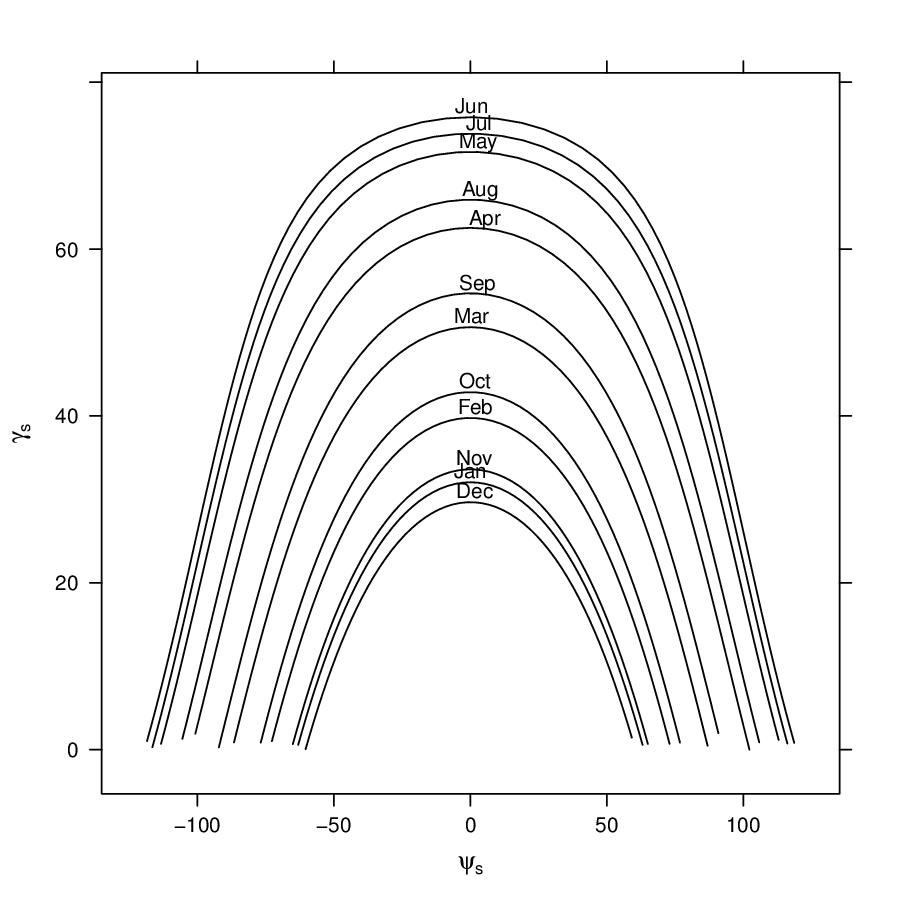
\includegraphics{solaR-006}

\par\end{centering}
\caption{\label{fig:AzimutAltura}Azimuth and height solar angles during the ``average days''.}
\end{figure}


These calculations can also be carried out for the whole year (figure \ref{fig:Declinacion}).

\begin{Schunk}
\begin{Sinput}
> BTd = fBTd(mode = "serie")
> solD <- fSolD(lat, BTd)
> summary(solD)
\end{Sinput}
\begin{Soutput}
     Index                 decl                eo              ws       
 Min.   :2011-01-01   Min.   :-0.40905   Min.   :0.967   Min.   :-1.91  
 1st Qu.:2011-04-02   1st Qu.:-0.27824   1st Qu.:0.976   1st Qu.:-1.80  
 Median :2011-07-02   Median : 0.01277   Median :0.999   Median :-1.58  
 Mean   :2011-07-02   Mean   : 0.00688   Mean   :1.000   Mean   :-1.58  
 3rd Qu.:2011-10-01   3rd Qu.: 0.29171   3rd Qu.:1.024   3rd Qu.:-1.35  
 Max.   :2011-12-31   Max.   : 0.40906   Max.   :1.035   Max.   :-1.24  
      Bo0d            EoT           
 Min.   : 4245   Min.   :-6.18e-02  
 1st Qu.: 5613   1st Qu.:-2.59e-02  
 Median : 8438   Median :-2.48e-03  
 Mean   : 8184   Mean   : 1.24e-05  
 3rd Qu.:10764   3rd Qu.: 2.16e-02  
 Max.   :11604   Max.   : 7.09e-02  
\end{Soutput}
\end{Schunk}


%
\begin{figure}
\begin{centering}
\begin{Schunk}
\begin{Sinput}
> p <- xyplot(solD$decl)
> print(p)
\end{Sinput}
\end{Schunk}
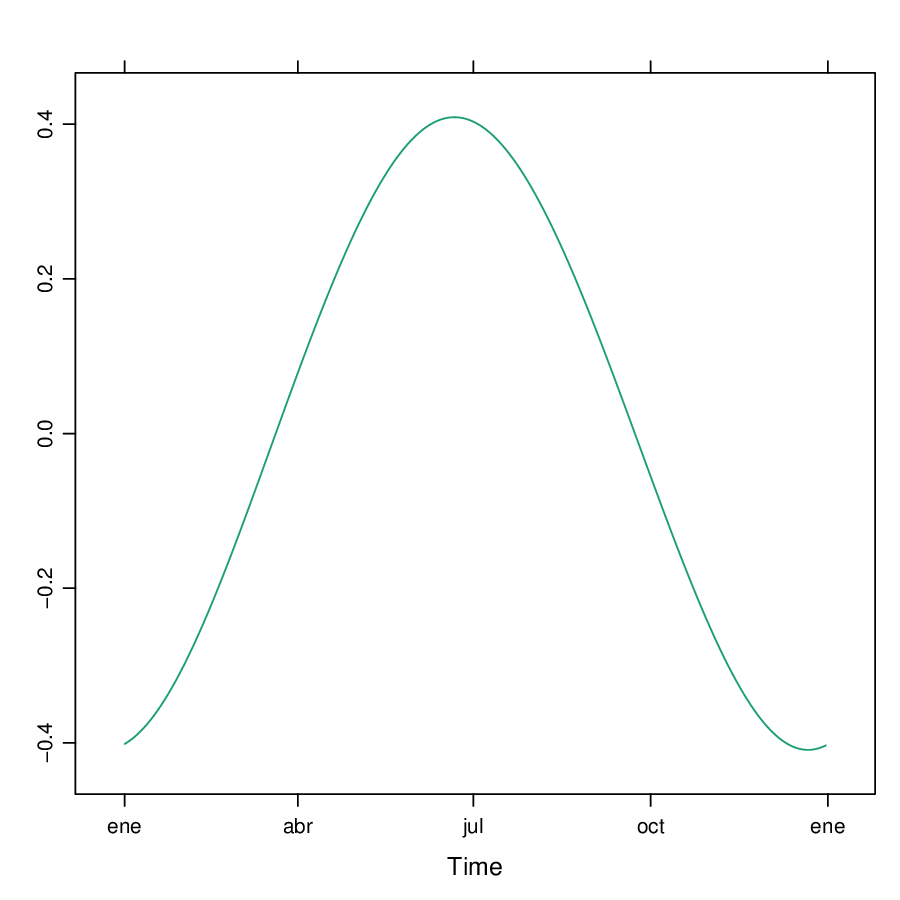
\includegraphics{solaR-008}
\par\end{centering}

\caption{Declination throughout the year\label{fig:Declinacion}}

\end{figure}

These two functions are included in a function,  \texttt{calcSol}. 
This function constructs an object of class  \texttt{Sol} containing in its slots 
the \texttt{zoo} objects created by \texttt{fSolD} and \texttt{fSolI}. 
This class owns methods for getting and displaying information (for example, \texttt{as.zooD, as.zooI, xyplot}).

There are three methods for the sun geometry calculations. These
methods are named as 'cooper' (the default in previous versions),
'spencer', 'michalsky' (the default in this version) and 'strous'. 
\begin{Schunk}
\begin{Sinput}
> lat = 37.2
> BTd = fBTd(mode = "serie")
> sol = calcSol(lat, BTd[100])
> print(as.zooD(sol))
\end{Sinput}
\begin{Soutput}
             decl     eo     ws Bo0d       EoT
2011-04-10 0.1383 0.9961 -1.677 9614 -0.004637
\end{Soutput}
\begin{Sinput}
> solStrous = calcSol(lat, BTd[100], method = "strous")
> print(as.zooD(solStrous))
\end{Sinput}
\begin{Soutput}
            decl     eo     ws Bo0d       EoT
2011-04-10 0.137 0.9961 -1.676 9603 -0.004637
\end{Soutput}
\begin{Sinput}
> solSpencer = calcSol(lat, BTd[100], method = "spencer")
> print(as.zooD(solSpencer))
\end{Sinput}
\begin{Soutput}
             decl     eo     ws Bo0d       EoT
2011-04-10 0.1336 0.9961 -1.673 9571 -0.004637
\end{Soutput}
\begin{Sinput}
> solCooper = calcSol(lat, BTd[100], method = "cooper")
> print(as.zooD(solCooper))
\end{Sinput}
\begin{Soutput}
             decl    eo     ws Bo0d       EoT
2011-04-10 0.1315 0.995 -1.671 9541 -0.004637
\end{Soutput}
\end{Schunk}



\chapter{Solar Radiation}

Values of global horizontal irradiation are commonly available either
as monthly averages of daily values or as a time series of daily
during one or several years.  The analysis of the performance of a PV
system starts from the transformation of the global horizontal
irradiation to global, diffuse and direct horizontal irradiance and
irradiation, and then irradiance and irradiation on the generator
surface.


\section{Irradiation and irradiance on the horizontal plane}

The function \texttt{fCompD} extracts the diffuse and direct
components from the daily global irradiation on a horizontal surface
by means of regressions between the clearness index and the diffuse
fraction parameters.  This function need the results from
\texttt{fSolD}, a set of values of global horizontal irradiation
($\si{\watthour\per\meter\squared}$), and the correlation between the
clearness index and the diffuse fraction.  The current version of
\texttt{solaR} includes several correlations (type
\texttt{help(corrFdKt)} for details).  Besides, the user may define a
particular correlation through the argument \texttt{f}.  Once again
for a certain day:

\begin{Schunk}
\begin{Sinput}
> BTd = fBTd(mode = "serie")
> SolD <- fSolD(lat, BTd[100])
> SolI <- fSolI(SolD, sample = "hour")
> G0d = zoo(5000, index(SolD))
> fCompD(SolD, G0d, corr = "Page")
\end{Sinput}
\begin{Soutput}
               Fd    Ktd  G0d  D0d  B0d
2011-04-10 0.4123 0.5201 5000 2062 2938
\end{Soutput}
\begin{Sinput}
> fCompD(SolD, G0d, corr = "CPR")
\end{Sinput}
\begin{Soutput}
               Fd    Ktd  G0d  D0d  B0d
2011-04-10 0.5658 0.5201 5000 2829 2171
\end{Soutput}
\end{Schunk}
and for the ``average days'':

\begin{Schunk}
\begin{Sinput}
> lat = 37.2
> G0dm = c(2.766, 3.491, 4.494, 5.912, 6.989, 7.742, 7.919, 7.027, 
     5.369, 3.562, 2.814, 2.179) * 1000
> Rad = readG0dm(G0dm, lat)
> solD <- fSolD(lat, fBTd(mode = "prom"))
> fCompD(solD, Rad, corr = "Page")
\end{Sinput}
\begin{Soutput}
               Fd    Ktd  G0d    D0d  B0d
2011-01-17 0.3412 0.5830 2766  943.8 1822
2011-02-14 0.3582 0.5679 3491 1250.6 2240
2011-03-15 0.3677 0.5596 4494 1652.5 2842
2011-04-15 0.3237 0.5985 5912 1914.0 3998
2011-05-15 0.2880 0.6301 6989 2012.8 4976
2011-06-10 0.2438 0.6692 7742 1887.1 5855
2011-07-18 0.2065 0.7022 7919 1635.1 6284
2011-08-18 0.2232 0.6875 7027 1568.1 5459
2011-09-18 0.2912 0.6272 5369 1563.7 3805
2011-10-19 0.3907 0.5392 3562 1391.7 2170
2011-11-18 0.3623 0.5643 2814 1019.6 1794
2011-12-13 0.4265 0.5075 2179  929.3 1250
\end{Soutput}
\end{Schunk}

Let's use \texttt{corr='user'} to define a function with the
correlation of Collares Pereira and Rabl \cite{Collares-Pereira.Rabl1979}. 
Obviously, we shall obtain the same result as with \texttt{corr='CPR'}.

\begin{Schunk}
\begin{Sinput}
> fKTd = function(x) {
     (0.99 * (x <= 0.17)) + (x > 0.17) * (1.188 - 2.272 * x + 
         9.473 * x^2 - 21.856 * x^3 + 14.648 * x^4)
 }
> fCompD(SolD, G0d, corr = "user", f = fKTd)
\end{Sinput}
\begin{Soutput}
               Fd    Ktd  G0d  D0d  B0d
2011-04-10 0.5658 0.5201 5000 2829 2171
\end{Soutput}
\end{Schunk}
                      
The daily profile of irradiance is obtained with the function \texttt{fCompI}. 
This function needs the information provided by \texttt{fCompD} and \texttt{fSolI} or \texttt{calcSol}. For example, the profiles for the ``average days'' are obtained with the next code (fig. \ref{fig:ComponentesIrradiancia}).

\begin{Schunk}
\begin{Sinput}
> lat = 37.2
> sol <- calcSol(lat, fBTd(mode = "prom"), sample = "hour", keep.night = FALSE)
> G0dm = c(2.766, 3.491, 4.494, 5.912, 6.989, 7.742, 7.919, 7.027, 
     5.369, 3.562, 2.814, 2.179) * 1000
> Ta = c(10, 14.1, 15.6, 17.2, 19.3, 21.2, 28.4, 29.9, 24.3, 18.2, 
     17.2, 15.2)
> BD <- readG0dm(G0dm = G0dm, Ta = Ta, lat = 37.2)
> compD <- fCompD(sol, BD, corr = "Page")
> compI <- fCompI(sol, compD)
\end{Sinput}
\end{Schunk}

%
\begin{figure}
\begin{centering}
\begin{Schunk}
\begin{Sinput}
> p <- xyplot(G0 + B0 + D0 ~ w | month, data = compI, type = "l", 
     auto.key = list(space = "right"))
> print(p)
\end{Sinput}
\end{Schunk}
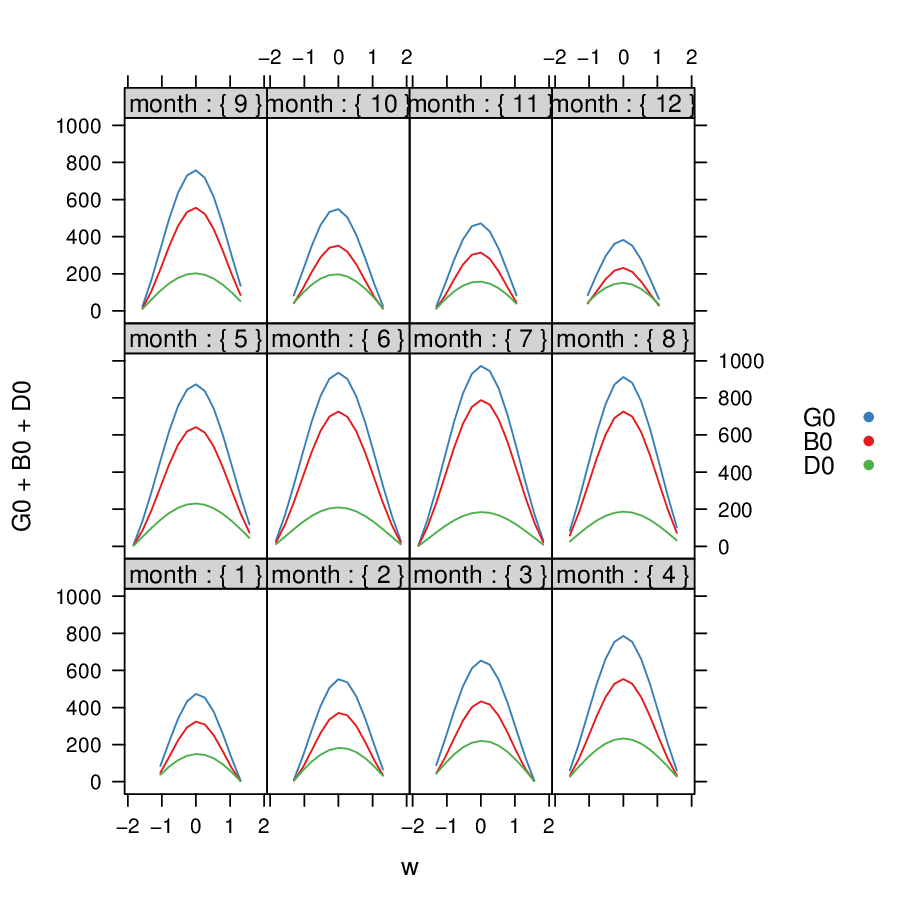
\includegraphics{solaR-014}
\par\end{centering}
\caption{Global, diffuse, and direct irradiance during the ``average days''.\label{fig:ComponentesIrradiancia}}
\end{figure}

\subsection{Meteorological data}

There are several functions to construct a \texttt{Meteo} object with radiation and temperature data.
For daily data, if it is stored in a local file or a  \texttt{data.frame}, the functions  \texttt{readBD} and \texttt{df2Meteo} are recommended, while \texttt{readG0dm} is indicated when only 12 monthly means are available. For intradaily data the correspondent functions are \texttt{readBDi} and \texttt{dfI2Meteo}. Besides, \texttt{zoo2Meteo} can construct a \texttt{Meteo} object from a \texttt{zoo} object both for daily and intradaily data.

For example, the \texttt{helios} dataset included in the package, obtained from \url{http://helios.ies-def.upm.es}, can be converted to a \texttt{Meteo} object with the next code:
\begin{Schunk}
\begin{Sinput}
> data(helios)
> names(helios) = c("date", "G0", "TempMax", "TempMin")
> bd = df2Meteo(helios, dates.col = "date", lat = 41, source = "helios-IES", 
     format = "%Y/%m/%d")
> summary(getData(bd))
\end{Sinput}
\begin{Soutput}
     Index                           G0           TempMax         TempMin      
 Min.   :2009-01-01 00:00:00   Min.   :  326   Min.   : 1.41   Min.   :-37.50  
 1st Qu.:2009-04-08 12:00:00   1st Qu.: 2523   1st Qu.:14.41   1st Qu.:  1.95  
 Median :2009-07-07 00:00:00   Median : 4746   Median :23.16   Median :  7.91  
 Mean   :2009-07-04 21:29:54   Mean   : 4812   Mean   :22.59   Mean   :  5.32  
 3rd Qu.:2009-10-03 12:00:00   3rd Qu.: 7140   3rd Qu.:31.06   3rd Qu.: 15.11  
 Max.   :2009-12-31 00:00:00   Max.   :11254   Max.   :38.04   Max.   : 24.80  
\end{Soutput}
\end{Schunk}

On the other hand, the function  \texttt{readSIAR} is able to download the meteorological data 
available at \url{www.marm.es/siar}.
This webpage provides daily measurements from a set of agroclimatic stations 
located in Spain. This function needs the code of the station and its province, 
and the start and end date. The codes of stations and provinces are stored at the
dataset \texttt{SIAR}. For example, there are several stations in Madrid:

\begin{Schunk}
\begin{Sinput}
> data(SIAR)
> Madrid <- subset(SIAR, Provincia == "Madrid")
> print(Madrid)
\end{Sinput}
\begin{Soutput}
    N_Estacion              Estacion N_Provincia Provincia           Comunidad
389          3              Aranjuez          28    Madrid Comunidad de Madrid
390          2               Arganda          28    Madrid Comunidad de Madrid
391          6              Chinchón          28    Madrid Comunidad de Madrid
392          4   Fuentidueña de Tajo          28    Madrid Comunidad de Madrid
393          5 San Martín de la Vega          28    Madrid Comunidad de Madrid
394        102       Villa del Prado          28    Madrid Comunidad de Madrid
       lon   lat Altitud
389 -3.600 40.02     551
390 -3.433 40.30     648
391 -3.400 40.13     749
392 -3.150 40.12     559
393 -3.567 40.20     515
394 -4.300 40.27     513
\end{Soutput}
\end{Schunk}

\texttt{readSIAR} constructs an object of class \texttt{Meteo}. The data is obtained with 
the method \texttt{getData}.  If only the irradiation series is needed, the method  \texttt{getG0} 
is recommended.

For example, let's obtain the 2009 data from the station at Aranjuez (fig. \ref{fig:Aranjuez}). 
It is important to note that the radiation measurements available at the webpage are
in  $\si{\mega\joule\per\meter\squared}$, but \texttt{readSIAR} converts the values to $\si{\watthour\per\meter\squared}$:

\begin{Schunk}
\begin{Sinput}
> Aranjuez <- readSIAR(28, 3, "01/01/2009", "31/12/2009")
\end{Sinput}
\begin{Soutput}
Downloading data from www.marm.es/siar...
\end{Soutput}
\end{Schunk}

\begin{figure}
  \centering
\begin{Schunk}
\begin{Sinput}
> p = xyplot(G0 ~ TempMedia | month, data = Aranjuez, type = c("p", 
     "r"))
> print(p)
\end{Sinput}
\end{Schunk}
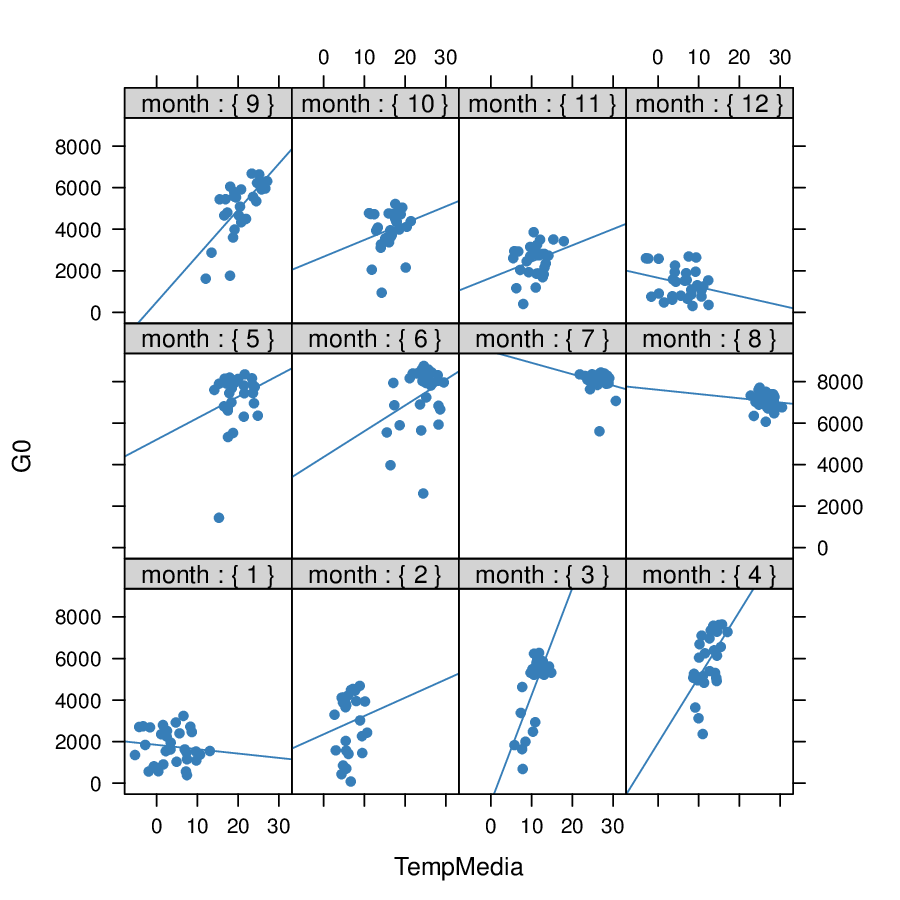
\includegraphics{solaR-018}
  \caption{Daily irradiation and mean temperature in the station of Aranjuez.}
  \label{fig:Aranjuez}
\end{figure}

This database includes information of maximum and minimum values of temperature. 
The function \texttt{fTemp} calculates a profile of the ambient temperature with this information
following the method proposed in \cite{Huld.Suri.ea2006}. 
The evolution of this synthetic temperature during March is displayed in the figure \ref{fig:Ta}.

\begin{Schunk}
\begin{Sinput}
> lat = 41
> sol = calcSol(lat, BTd = indexD(Aranjuez), sample = "hour")
> Temp <- fTemp(sol, Aranjuez)